% questions.tex —— 2021 年·新高考Ⅱ卷 · 题目内容片段（无答案）
% 由 tools/generate_projects.py 依来源总账自 2021/2021_数学真题_新高考Ⅱ_试题.md 生成，勿手改（改源 MD 后重跑）


\begin{gknotice}
\textbf{结构提示}：本卷为 \textbf{22 题制}（2024 年起改为 19 题制），宜按知识点抽题使用，不宜整套限时模拟。

\textbf{适用省份}：辽宁、重庆、海南

\textbf{来源说明}：试题原文取自 deekur/gaokaomath（commit \texttt{34c13a6}，CC BY 4.0）之「2021新高考2」PDF，逐题照图转录。
\end{gknotice}

\par\medskip

\gkpart{一、单选题}

\begin{gktip}
本题共 8 小题，每小题 5 分，共 40 分。在每小题给出的四个选项中，只有一项是符合题目要求的。
\end{gktip}

\begin{question}
\gkti{1}复数 $\dfrac{2-\mathrm i}{1-3\mathrm i}$ 在复平面内对应的点所在的象限为（　　）

\begin{gkopts}(4)
\task A．第一象限
\task B．第二象限
\task C．第三象限
\task D．第四象限
\end{gkopts}

\end{question}
\begin{question}
\gkti{2}若全集 $U=\{1,2,3,4,5,6\}$，集合 $A=\{1,3,6\}$，$B=\{2,3,4\}$，则 $A\cap\left(\complement_U B\right)=$（　　）

\begin{gkopts}(4)
\task A．$\{3\}$
\task B．$\{1,6\}$
\task C．$\{5,6\}$
\task D．$\{1,3\}$
\end{gkopts}

\end{question}
\begin{question}
\gkti{3}若抛物线 $y^{2}=2px\ (p>0)$ 的焦点到直线 $y=x+1$ 的距离为 $\sqrt2$，则 $p=$（　　）

\begin{gkopts}(4)
\task A．$1$
\task B．$2$
\task C．$2\sqrt2$
\task D．$4$
\end{gkopts}

\end{question}
\begin{question}
\gkti{4}北斗三号全球卫星导航系统是我国航天事业的重要成果。在卫星导航系统中，地球静止同步轨道卫星的轨道位于地球赤道所在平面，轨道高度为 $36000\ \mathrm{km}$（轨道高度是指卫星到地球表面的最短距离），把地球看成一个球心为 $O$，半径 $r$ 为 $6400\ \mathrm{km}$ 的球，其上点 $A$ 的纬度是指 $OA$ 与赤道所在平面所成角的度数，地球表面能直接观测到的一颗地球静止同步轨道卫星的点的纬度的最大值记为 $\alpha$，该卫星信号覆盖的地球表面面积 $S=2\pi r^{2}(1-\cos\alpha)$（单位：$\mathrm{km}^{2}$），则 $S$ 占地球表面积的百分比约为（　　）

\begin{gkopts}(4)
\task A．$26\%$
\task B．$34\%$
\task C．$42\%$
\task D．$50\%$
\end{gkopts}

\end{question}
\begin{question}
\gkti{5}正四棱台的上、下底面的边长为 $2$，$4$，侧棱长为 $2$，则其体积为（　　）

\begin{gkopts}(2)
\task A．$56$
\task B．$28\sqrt2$
\task C．$\dfrac{56}3$
\task D．$\dfrac{28\sqrt2}3$
\end{gkopts}

\end{question}
\begin{question}
\gkti{6}某物理量的测量结果服从正态分布 $N\left(10,\sigma^{2}\right)$，则下列结论中不正确的是（　　）

\begin{gkopts}(1)
\task A．$\sigma$ 越小，该物理量一次测量结果落在 $(9.9,10.1)$ 内的概率越大
\task B．该物理量一次测量结果大于 $10$ 的概率为 $0.5$
\task C．该物理量一次测量结果小于 $9.99$ 的概率与大于 $10.01$ 的概率相等
\task D．该物理量一次测量结果落在 $(9.9,10.2)$ 内的概率与落在 $(10,10.3)$ 内的概率相等
\end{gkopts}

\end{question}
\begin{question}
\gkti{7}若 $a=\log_52$，$b=\log_83$，$c=\dfrac12$，则（　　）

\begin{gkopts}(4)
\task A．$c<b<a$
\task B．$b<a<c$
\task C．$a<c<b$
\task D．$a<b<c$
\end{gkopts}

\end{question}
\begin{question}
\gkti{8}设函数 $f(x)$ 的定义域为 $\mathbf R$，且 $f(x+2)$ 为偶函数，$f(2x+1)$ 为奇函数，则（　　）

\begin{gkopts}(2)
\task A．$f\left(-\dfrac12\right)=0$
\task B．$f(-1)=0$
\task C．$f(2)=0$
\task D．$f(4)=0$
\end{gkopts}

\par\medskip

\end{question}
\gkpart{二、多选题}

\begin{gktip}
本题共 4 小题，每小题 5 分，共 20 分。全部选对得 5 分，部分选对得 2 分，有选错得 0 分。
\end{gktip}

\begin{question}
\gkti{9}下列统计量中可用于度量样本 $x_1,x_2,\cdots,x_n$ 离散程度的有（　　）

\begin{gkopts}(2)
\task A．$x_1,x_2,\cdots,x_n$ 的标准差
\task B．$x_1,x_2,\cdots,x_n$ 的中位数
\task C．$x_1,x_2,\cdots,x_n$ 的极差
\task D．$x_1,x_2,\cdots,x_n$ 的平均数
\end{gkopts}

\Needspace{0.4\textheight}
\end{question}
\begin{question}
\gkti{10}如图，下列各正方体中，$O$ 为下底面的中心，$M$，$N$ 为顶点，$P$ 为所在棱的中点，则满足 $MN\perp OP$ 的是（　　）
\nopagebreak[4]
\begin{center}% 2021 新高考Ⅱ卷 10：四个正方体选项图 (A)(B)(C)(D)
% 绘制依据：源 PDF（deekur/gaokaomath 2021新高考2）第 1 页原图，经 260dpi 裁剪逐图核对点位。
% 统一设棱长 2：前面正方形 (0,0)-(2,2)，后向偏移 (0.85,0.5)；O 为下底面中心。
% 画布坐标 = (x + 0.425y, z + 0.25y)，立体坐标系：x 右、y 后、z 上。
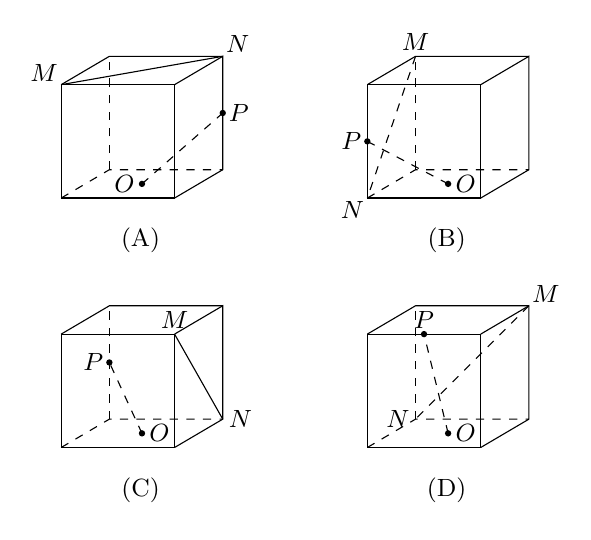
\begin{tikzpicture}[scale=0.72, font=\small]
  % ---------- (A)：M(0,0,2) 左前上，N(2,2,2) 右后上，P(2,2,1) 右后竖棱中点；MN 上底面对角线 ----------
  \begin{scope}
    \draw (0,0) rectangle (2,2);
    \draw (2,0) -- (2.85,0.5) -- (2.85,2.5) -- (2,2);
    \draw (0,2) -- (0.85,2.5) -- (2.85,2.5);
    \draw[dashed] (0,0) -- (0.85,0.5) -- (2.85,0.5);
    \draw[dashed] (0.85,0.5) -- (0.85,2.5);
    \coordinate (M) at (0,2);      \coordinate (N) at (2.85,2.5);
    \coordinate (P) at (2.85,1.5); \coordinate (O) at (1.425,0.25);
    \draw (M) -- (N);
    \draw[dashed] (O) -- (P);
    \fill (P) circle (1.6pt); \fill (O) circle (1.6pt);
    \node[above left, inner sep=1pt] at (M) {$M$};
    \node[above right, inner sep=1pt] at (N) {$N$};
    \node[right, inner sep=2pt] at (P) {$P$};
    \node[left, inner sep=2.5pt] at (O) {$O$};
    \node at (1.4,-0.75) {(A)};
  \end{scope}
  % ---------- (B)：M(0,2,2) 左后上，N(0,0,0) 左前下，P(0,0,1) 左前竖棱中点；MN 左侧面对角线（被遮挡） ----------
  \begin{scope}[xshift=5.4cm]
    \draw (0,0) rectangle (2,2);
    \draw (2,0) -- (2.85,0.5) -- (2.85,2.5) -- (2,2);
    \draw (0,2) -- (0.85,2.5) -- (2.85,2.5);
    \draw[dashed] (0,0) -- (0.85,0.5) -- (2.85,0.5);
    \draw[dashed] (0.85,0.5) -- (0.85,2.5);
    \coordinate (M) at (0.85,2.5); \coordinate (N) at (0,0);
    \coordinate (P) at (0,1);      \coordinate (O) at (1.425,0.25);
    \draw[dashed] (M) -- (N);
    \draw[dashed] (O) -- (P);
    \fill (P) circle (1.6pt); \fill (O) circle (1.6pt);
    \node[above, inner sep=2pt] at (M) {$M$};
    \node[below left, inner sep=1pt] at (N) {$N$};
    \node[left, inner sep=2pt] at (P) {$P$};
    \node[right, inner sep=2.5pt] at (O) {$O$};
    \node at (1.4,-0.75) {(B)};
  \end{scope}
  % ---------- (C)：M(2,0,2) 右前上，N(2,2,0) 右后下，P(0,2,1) 左后竖棱（隐藏棱）中点；MN 右侧面对角线 ----------
  \begin{scope}[yshift=-4.4cm]
    \draw (0,0) rectangle (2,2);
    \draw (2,0) -- (2.85,0.5) -- (2.85,2.5) -- (2,2);
    \draw (0,2) -- (0.85,2.5) -- (2.85,2.5);
    \draw[dashed] (0,0) -- (0.85,0.5) -- (2.85,0.5);
    \draw[dashed] (0.85,0.5) -- (0.85,2.5);
    \coordinate (M) at (2,2);      \coordinate (N) at (2.85,0.5);
    \coordinate (P) at (0.85,1.5); \coordinate (O) at (1.425,0.25);
    \draw (M) -- (N);
    \draw[dashed] (O) -- (P);
    \fill (P) circle (1.6pt); \fill (O) circle (1.6pt);
    \node[above, inner sep=2pt] at (M) {$M$};
    \node[right, inner sep=2pt] at (N) {$N$};
    \node[left, inner sep=2pt] at (P) {$P$};
    \node[right, inner sep=2.5pt] at (O) {$O$};
    \node at (1.4,-0.75) {(C)};
  \end{scope}
  % ---------- (D)：M(2,2,2) 右后上，N(0,2,0) 左后下，P(1,0,2) 前上棱中点；MN 后侧面对角线（被遮挡） ----------
  \begin{scope}[xshift=5.4cm, yshift=-4.4cm]
    \draw (0,0) rectangle (2,2);
    \draw (2,0) -- (2.85,0.5) -- (2.85,2.5) -- (2,2);
    \draw (0,2) -- (0.85,2.5) -- (2.85,2.5);
    \draw[dashed] (0,0) -- (0.85,0.5) -- (2.85,0.5);
    \draw[dashed] (0.85,0.5) -- (0.85,2.5);
    \coordinate (M) at (2.85,2.5); \coordinate (N) at (0.85,0.5);
    \coordinate (P) at (1,2);      \coordinate (O) at (1.425,0.25);
    \draw[dashed] (M) -- (N);
    \draw[dashed] (O) -- (P);
    \fill (P) circle (1.6pt); \fill (O) circle (1.6pt);
    \node[above right, inner sep=1pt] at (M) {$M$};
    \node[left, inner sep=2pt] at (N) {$N$};
    \node[above, inner sep=2pt] at (P) {$P$};
    \node[right, inner sep=2.5pt] at (O) {$O$};
    \node at (1.4,-0.75) {(D)};
  \end{scope}
\end{tikzpicture}\end{center}
\nopagebreak[4]
\end{question}
\begin{question}
\gkti{11}已知直线 $l:ax+by-r^{2}=0$ 与圆 $C:x^{2}+y^{2}=r^{2}$，点 $A(a,b)$，则下列说法正确的是（　　）

\begin{gkopts}(1)
\task A．若点 $A$ 在圆 $C$ 上，则直线与圆 $C$ 相切
\task B．若点 $A$ 在圆 $C$ 内，则直线 $l$ 与圆 $C$ 相离
\task C．若点 $A$ 在圆 $C$ 外，则直线 $l$ 与圆 $C$ 相离
\task D．若点 $A$ 在直线 $l$ 上，则直线 $l$ 与圆 $C$ 相切
\end{gkopts}

\end{question}
\begin{question}
\gkti{12}设正整数 $n=a_0\cdot2^{0}+a_1\cdot2^{1}+\cdots+a_{k-1}\cdot2^{k-1}+a_k\cdot2^{k}$，其中 $a_i\in\{0,1\}$，记 $\omega(n)=a_0+a_1+\cdots+a_k$。则（　　）

\begin{gkopts}(2)
\task A．$\omega(2n)=\omega(n)$
\task B．$\omega(2n+3)=\omega(n)+1$
\task C．$\omega(8n+5)=\omega(4n+3)$
\task D．$\omega\left(2^{n}-1\right)=n$
\end{gkopts}

\par\medskip

\end{question}
\gkpart{三、填空题}

\begin{gktip}
本题共 4 小题，每小题 5 分，共 20 分。
\end{gktip}

\begin{question}
\gkti{13}已知双曲线 $C:\dfrac{x^{2}}{a^{2}}-\dfrac{y^{2}}{b^{2}}=1\ (a>0,b>0)$ 的离心率 $e=2$，则双曲线 $C$ 的渐近线方程为 \gkblank{}．

\end{question}
\begin{question}
\gkti{14}写出一个同时具有下列性质①②③的函数 $f(x)=$ \gkblank{}．

  ① $f\left(x_1x_2\right)=f\left(x_1\right)f\left(x_2\right)$；
  ② 当 $x\in(0,+\infty)$ 时，$f'(x)>0$；
  ③ $f'(x)$ 是奇函数．

\end{question}
\begin{question}
\gkti{15}已知向量 $\boldsymbol a+\boldsymbol b+\boldsymbol c=\boldsymbol 0$，$|\boldsymbol a|=1$，$|\boldsymbol b|=|\boldsymbol c|=2$，则 $\boldsymbol a\cdot\boldsymbol b+\boldsymbol b\cdot\boldsymbol c+\boldsymbol c\cdot\boldsymbol a=$ \gkblank{}．

\end{question}
\begin{question}
\gkti{16}已知函数 $f(x)=\left|\mathrm e^{x}-1\right|$，$x_1<0$，$x_2>0$，函数 $f(x)$ 的图象在点 $A\left(x_1,f\left(x_1\right)\right)$ 和点 $B\left(x_2,f\left(x_2\right)\right)$ 处的两条切线互相垂直，且分别交 $y$ 轴于 $M$，$N$ 两点，则 $\dfrac{|AM|}{|BN|}$ 的取值范围是 \gkblank{}．

\par\medskip

\end{question}
\gkpart{四、解答题}

\begin{gktip}
本题共 6 小题，共 70 分。解答应写出文字说明、证明过程或演算步骤。
\end{gktip}

\begin{question}
\gkti{17}\textbf{（10 分）} 记 $S_n$ 是公差不为 $0$ 的等差数列 $\left\{a_n\right\}$ 的前 $n$ 项和，若 $a_3=S_5$，$a_2a_4=S_4$．

  (1) 求数列 $\left\{a_n\right\}$ 的通项公式；

  (2) 求使 $S_n>a_n$ 成立的 $n$ 的最小值．

\end{question}
\begin{question}
\gkti{18}\textbf{（12 分）} 在 $\triangle ABC$ 中，角 $A$，$B$，$C$ 所对的边分别为 $a$，$b$，$c$，$b=a+1$，$c=a+2$．

  (1) 若 $2\sin C=3\sin A$，求 $\triangle ABC$ 的面积；

  (2) 是否存在正整数 $a$，使得 $\triangle ABC$ 为钝角三角形？若存在，求 $a$；若不存在，说明理由．

\Needspace{0.4\textheight}
\end{question}
\begin{question}
\gkti{19}\textbf{（12 分）} 如图，在四棱锥 $Q\text{-}ABCD$ 中，底面 $ABCD$ 是正方形，$AD=2$，$QD=QA=\sqrt5$，$QC=3$．
\nopagebreak[4]
\begin{center}% 2021 新高考Ⅱ卷 19：四棱锥 Q-ABCD，底面为正方形
% 绘制依据：源 PDF 原图方位——A 后方偏左、B 左前、C 右前、D 右；QA、QD 为虚线。
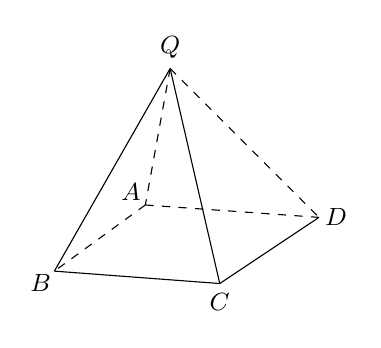
\begin{tikzpicture}[scale=1.05, font=\small]
  \coordinate (Q) at (1.75,2.6);
  \coordinate (A) at (1.45,0.95);
  \coordinate (B) at (0.35,0.15);
  \coordinate (C) at (2.35,0);
  \coordinate (D) at (3.55,0.8);
  \draw (Q) -- (B)  (Q) -- (C);
  \draw (B) -- (C) -- (D);
  \draw[dashed] (Q) -- (A)  (Q) -- (D);
  \draw[dashed] (A) -- (B)  (A) -- (D);
  \node[above] at (Q) {$Q$};
  \node[above left, inner sep=1.5pt] at (A) {$A$};
  \node[below left, inner sep=1pt] at (B) {$B$};
  \node[below] at (C) {$C$};
  \node[right, inner sep=2pt] at (D) {$D$};
\end{tikzpicture}\end{center}
\nopagebreak[4]
  (1) 证明：平面 $QAD\perp$ 平面 $ABCD$；

  (2) 求二面角 $B\text{-}QD\text{-}A$ 的余弦值．

\end{question}
\begin{question}
\gkti{20}\textbf{（12 分）} 已知椭圆 $C:\dfrac{x^{2}}{a^{2}}+\dfrac{y^{2}}{b^{2}}=1\ (a>b>0)$，右焦点为 $F\left(\sqrt2,0\right)$，其离心率为 $\dfrac{\sqrt6}3$．

  (1) 求椭圆 $C$ 的方程；

  (2) 设 $M$，$N$ 是椭圆 $C$ 上的两点，直线 $MN$ 与曲线 $x^{2}+y^{2}=b^{2}\ (x>0)$ 相切．证明：$M$，$N$，$F$ 三点共线的充要条件是 $|MN|=\sqrt3$．

\end{question}
\begin{question}
\gkti{21}\textbf{（12 分）} 一种微生物群体可以经过自身繁殖不断生存下来，设一个这种微生物为第 $0$ 代，经过一次繁殖后为第 $1$ 代，再经过一次繁殖后为第 $2$ 代……该微生物每代繁殖的个数是相互独立的且有相同的分布列，设 $X$ 表示 $1$ 个微生物个体繁殖下一代的个数，$P(X=i)=p_i>0\ (i=0,1,2,3)$．

  (1) 已知 $p_0=0.4$，$p_1=0.3$，$p_2=0.2$，$p_3=0.1$，求 $E(X)$；

  (2) 设 $p$ 表示该种微生物经过多代繁殖后临近灭绝的概率，$p$ 是关于 $x$ 的方程：$p_0+p_1x+p_2x^{2}+p_3x^{3}=x$ 的一个最小正实根，求证：当 $E(X)\le1$ 时，$p=1$，当 $E(X)>1$ 时，$p<1$；

  (3) 根据你的理解说明 (2) 问结论的实际含义．

\end{question}
\begin{question}
\gkti{22}\textbf{（12 分）} 已知函数 $f(x)=(x-1)\mathrm e^{x}-ax^{2}+b$．

  (1) 讨论 $f(x)$ 的单调性；

  (2) 从下面两个条件中任选一个作为已知条件，证明：$f(x)$ 有一个零点．

  ① $\dfrac12<a\le\dfrac{\mathrm e^{2}}2$，$b>2a$；

  ② $0<a<\dfrac12$，$b\le2a$．

\par\medskip

\begin{gktip}
\textbf{试题来源}：deekur/gaokaomath（commit \texttt{34c13a6}，CC BY 4.0）之「2021新高考2」PDF。
\end{gktip}

\end{question}